%
% einleitung.tex -- Einleitung zum Skript ueber Differentialgleichungen
%
% (c) 2015 Prof Dr Andreas Mueller, Hochschule Rapperswil
%
\chapter{Einleitung\label{chapter:einleitung}}
\lhead{Einleitung}
\rhead{}
In XKCD 135 (Abbildung~\ref{einleitung:xkcd135})
\index{XKCD}%
\index{Munroe, Randall}%
beschreibt Randall Munroe erdachte Aufgaben "uber die
Jagdgewohnheiten von Velociraptoren, Fragen, bei denen es um Leben
und Tod geht.
Die Aufgaben k"onnen zwar ohne Differentialgleichungen gel"ost
werden, aber sie k"onnen leicht zu noch spannenderen Aufgaben
verallgemeinert werden, die nicht ohne die Kenntnisse von 
Differentialgleichungen gel"ost werden k"onnen.
Dies zeigt, dass die Kenntnis der L"osungsverfahren von Differentialgleichungen
eine Frage von Leben und Tod ist.

\index{Newton!Isaac}
Isaac Newtons Grundgesetze der Dynamik sind die ersten Beispiele
\index{Newton, Isaac}
von Differentialgleichungen.
Sein erstes Gesetz besagt:
\index{Newton!erstes Gesetz von}
\begin{quote}
\em
Ein K"orper verharrt im Zustand der Ruhe oder der gleichf"ormigen Translation,
sofern er nicht durch einwirkende Kr"afte zur "Anderung seines Zustands
gezwungen wird.
\end{quote}
In der Abwesenheit von Kr"aften ver"andert sich die Geschwindigkeit nicht,
oder 
\[
\frac{d}{dt}\vec{v}=0,
\]
wobei $\vec{v}$ der Vektor der Geschwindigkeit ist.
Das erste Gesetz oder Tr"agheitsprinzip wurde schon von Galileo Galilei
formuliert.
\index{Tragheitsprinzip@Tr\"agheitsprinzip}%

\begin{figure}
\centering
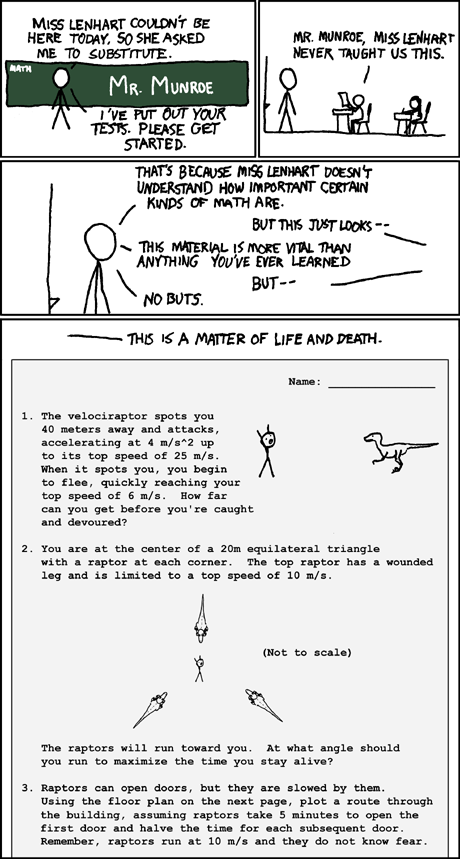
\includegraphics[width=0.7\hsize]{chapters/substitute.png}
\caption{xkcd 135 mit von Randall Munroe erdachten Aufgaben "uber die
Jagdgewohnheiten von Velociraptoren.
\label{einleitung:xkcd135}}
\end{figure}%


Das zweite Gesetz besagt:
\index{Newton!zweites Gesetz von}
\begin{quote}
\em
Die "Anderung der Bewegung ist der Einwirkung der bewegenden Kraft
proportional und geschieht nach der Richtung derjenigen geraden Linie,
nach welcher jene Kraft wirkt.
\end{quote}
Mit {\em Bewegung}
meint Newton den Impuls $\vec{p}=m\vec{v}$,
\index{Impuls}%
das zweite Gesetz wird in moderner Schreibweise
\[
\frac{d}{dt}(m\vec{v}) = \vec{F}.
\]
In beiden F"allen wird die "Anderung einer Zustandsvariablen, n"amlich
des Impulses, mit dem aktuellen Zustand, typischerweise der Position,
verkn"upft.
Die Newtonschen Bewegungsgesetze sind Differentialgleichungen.
\index{Newton!Bewegungsgesetz}

Das neue Werkzeug der Infinitesimalrechnung bescherte der exakten
Naturwissenschaft eine F"ulle neuer Probleml"osungen, die alle
nach dem gleichen Prinzip vorgingen.
\begin{enumerate}
\item
Finde Differentialgleichungen zwischen den Zustandsvariablen
eines Systems, "ublicherweise durch Anwendung des zweiten
Newtonschen Gesetztes.
\item
L"ose die Differentialgleichungen und
ziehe Schl"usse.
\end{enumerate}
Die besondere Leistung dieses Plans ist, dass die Differentialgleichung
nur Konzepte miteinander verkn"upft, die in einem Punkt definiert sind.
Die Beschleunigung in einem Punkt wird mit den in diesem Punkt wirkenden
Kr"aften verkn"upft.
Erst bei der L"osung der Differentialgleichung wird der globale Verlauf
der gesuchten Funktion rekonstruiert.
Die Theorie der Differentialgleichungen liefert also ein Verfahren
f"ur den {\em "Ubergang vom Lokalen zum Globalen}.
In diesem Skript geht es weniger um analytische Methoden, wie man
L"osungsformeln f"ur Differentialgleichungen finden kann, sondern
vielmehr um die Frage, was sich "uberhaupt "uber die globale L"osung
sagen l"asst, wenn man von der durch die in der Differentialgleichung 
codierten lokalen Information ausgeht.

Es zeigte sich bald, dass viele Differentialgleichungen
keine L"osungen haben, die sich mit den bisher bekannten Funktionen
ausdr"ucken lassen.
Man behalf sich kurzerhand damit, neue Funktionen zu definieren, 
die bald Anwendungen in den verschieden Gebieten der Technik fanden.
Die Bessel-Funktionen sind mittlerweile so wichtig, dass sie in keiner
Computer-Bibliothek f"ur mathematische Funktionen fehlen d"urfen.
\index{Bessel-Funktionen}%

Die Herkunft der Kr"afte wird in den Newtonschen Gesetzen nicht weiter
gekl"art, doch Newton selbst beschreibt mit seinem Gravitationsgesetz
die Herkunft der Kr"afte, die die Planeten im Sonnensystem auf ihren Bahnen
halten.
\index{Gravitationsgesetz}%
\index{Kepler, Johannes}%
\index{Kepler-Bahn}%
\index{Sonnensystem}%
Er zeigt, dass die Keplerschen Ellipsenbahnen L"osungen seiner
Bewegungsgleichungen sind.
Die rein kinematische Beschreibung durch Kepler machte einem
dynamischen Verst"andnis Platz, welches nun auch die gegenseitigen
Einfl"usse der Planeten aufeinander zu berechnen gestattete.
Und tats"achlich war Newton der erste, der sich dar"uber Gedanken
machte, wie sich das Sonnensystem "uber lange Zeit entwickeln w"urde.
Seine Schlussfolgerung aus seinen aus heutiger Sicht rudiment"aren
Untersuchungen: das Sonnensystem ist instabil, "uber Jahrmillionen 
werden die Planeten in den interstellaren Raum geschleudert werden.
\index{Ellipsenbahn}

Die industrielle Revolution brachte eine Vielzahl von Maschinen,
\index{industrielle Revolution}%
die automatisch geregelt werden mussten.
Ingenieure entwickelten eine ganze Reihe von einfallsreichen L"osungen,
doch erst in der Mitte des 19.~Jahrhunderts konnten Physiker diese
Apparaturen mit Differentialgleichungen erkl"aren und ihre Stabilit"at
untersuchen.
Im zwanzigsten Jahrhundert reiften die mathematischen Hilfsmittel
soweit, dass auch instabile L"osungen untersucht werden konnten,
wie sie bei nichtlinearen Differentialgleichungen auftreten.
Mittlerweile ist das Auftreten von Instabilit"aten recht gut verstanden
und klassifiziert. 
Die Technik der Linearisierung erm"oglicht zum Beispiel die
Hopf-Bifurkation zu verstehen.
\index{Hopf-Bifurkation}%
\index{Bifurkation!Hopf}%
Auch die Sattel-Knoten-Bifurkation und die Heugabel-Bifurkation
lassen sich in Anwendungen finden.
\index{Bifurkation!Sattel-Knoten-}%
\index{Sattel-Knoten-Bifurkation}%
\index{Bifurkation!Heugabel-}%
\index{Heugabel-Bifurkation}%
Und die Chaos-Theorie versteht sogar, wie "uber eine Kaskade von
Bifurkationen die Bewegung eines Systems jede Vorhersagbarkeit verliert,
es bewegt sich chaotisch.
\index{Chaos}%

In vielen F"allen l"asst sich eine Differentialgleichung erst dann
verstehen, wenn man in komplexen Zahlen arbeitet. 
Die Hopf-Bifurkation tritt zum Beispiel genau dann auf, wenn eine
Bedingung "uber die komplexen Eigenwerte des linearisierten Systems
erf"ullt ist.
Im Anhang~\ref{appendix:komplexezahlen} werden die grundlegenden Eigenschaften
komplexer Zahlen zusammengestellt.

Im Kapitel~2 sollen zun"achst Begriffe und Notation festgelegt werden,
danach sollen einige analytische Grundtechniken vermittelt werden.
Im Kapitel~3 wird gezeigt, wie Differentialgleichungen numerisch
gel"ost werden k"onnen.

Bei der L"osung von Randwertproblemen f"ur gew"ohnliche Differentialgleichungen
ist der Newton-Algorithmus oft ein zweckm"assiges Hilfsmittel.
Zusammen mit der im Kapitel~2 hergeleiteten Differentialgleichung f"ur
die Ableitung nach den Anfangsbedingungen liefert er ein sehr schnelles
Verfahren.
Er ist allerdings nicht spezifisch f"ur Differentialgleichungen, und
wird daher im Anhang~\ref{chapter:newton} behandelt.

Die Potenzreihenmethode ist Inhalt von Kapitel~4. 
Den sehr wichtigen Spezialfall linearer Differentialgleichungen
behandelt Kapitel~5 genauer.
Geometrische Eigenschaften von Vektorfeld und L"osung lassen oft
bereits ausreichend genaue Aussagen "uber die L"osung zu,  dies wird
im Kapitel~6 gezeigt.
Im Komplexen wird die Theorie sehr viel reichhaltiger, Kapitel~7 gibt
einen "Uberblick "uber die komplexe Analysis.

In der Praxis beeinflussen oft stochastische Prozesse die L"osung einer
Differentialgleichung, zum Beispiel das Rauschen in einer elektronischen
Schaltung.
Kapitel~8 zeigt, wie man die Theorie der gew"ohnlichen Differentialgleichungen
erweitern kann, dass Prozesse wie das Rauschen korrekt modelliert 
werden k"onnen, und Fragen "uber erwartete L"osung und Varianz
derselben zuverl"assig beantwortet werden k"onnen\footnote{Dieses Thema
wurde nur im Master-Seminar behandelt.}.

%Weitere Literaturhinweise im Literaturverzeichnis auf
%Seite~\pageref{skript:literatur}.

